\chapter{Evaluation}
\label{chapter:evaluation}
In this chapter, we will evaluate and discuss the performance of our polymorphic interpreter on six microbenchmarks.
We use an existing set of benchmarks from \cite{scala:miniboxing} as they exercise many features of the Scala runtime that require specialization to perform optimally.
We will evaluate the performance of these benchmarks on the monomorphic interpreter and Scala bytecode on GraalVM as points of comparison for relative performance.
Finally, we discuss the results of the benchmarks, examine the causes of performance deficiencies, and how our implementation resolves them.

\section{Benchmarks}
\begin{figure}[!htb]
	\begin{minted}{scala}
	class ArrayBuffer[T] {
		protected def initialSize: Int = 16
		var size0 = 0
		var array: Array[T] = newArray[T](Math.max(initialSize, 1))
		
		def length: Int = size0
		
		private def get(i: Int): T = array(i)
		private def set(i: Int, elem: T): Unit = array(i) = elem
		
		def contains(elem: T): Boolean = {
			var i = 0
			while (i < size0) {
				if (array(i) == elem) return true
				i += 1
			}
			false
		}
		
		def reverse(): Unit = {
			var pos = 0
			while (pos * 2 < size0) {
				swap(pos, size0 - pos - 1) // swaps two elements in the array
				pos += 1
			}
		}
		
		def append(elem: T): Unit = {
			val newSize0 = size0 + 1
			ensureSize(newSize0)
			set(size0, elem)
			size0 = newSize0
		}
		
		// Ensure that the internal array has at least `n` cells. 
		def ensureSize(n: Int): Unit = {
			val arrayLength: Long = array.length // Use a Long to prevent overflows
			if (n > arrayLength) {
				var newSize: Long = arrayLength * 2
				while (n > newSize)
					newSize = newSize * 2
				// Clamp newSize to Int.MaxValue
				if (newSize > lang.Int.MaxValue) newSize = lang.Int.MaxValue
				
				val resized = newArray[T](newSize.toInt)
				var i = 0
				while (i < size0) {
					resized(i) = get(i)
					i += 1
				}
				array = resized
			}
		}
	\end{minted}
	\caption{Code of the \scalainline{ArrayBuffer} benchmark.}
	\label{example:arraybuffer-benchmark}
\end{figure}

In this section, we will introduce an additional program on top of our running example for benchmarking.
We will also summarize the motivations for selecting these benchmarks from \cite{scala:miniboxing}.

Each microbenchmark exercises unique polymorphic operations which are typically performance bottlenecks\cite{scala:collections-optimization}\cite{scala:dacapo} in Scala programs.
The \scalainline{ArrayBuffer} class implements a resizable buffer backed by an array.
It contains three microbenchmarks that stress polymorphic operations in the context of contiguous memory access.

The \scalainline{List} class is the implementation of a linked list that we have used as the running example in this thesis.
We use the \scalainline{List} class to evaluate polymorphic operations in the context of random heap access.
Like the \scalainline{ArrayBuffer} benchmarks, there is an \scalainline{append} and \scalainline{contains} microbenchmark.
We will use lists to test the performance of polymorphic hash computations using \scalainline{List.hashCode}.

\section{Methodology}

Performance measurement of just-in-time compiled programs is an infamously difficult issue\cite{java:performance-analysis}\cite{java:statistically-rigor-performance-analysis}.
Many non-deterministic effects, such as speculative optimization, garbage collection, and thread scheduling, affect the performance of programs executing on the Java Virtual Machine.
As a result, the JVM must be \textit{warmed up} before measuring program performance.
A benchmarking routine is warmed up with several iterations of invocations for profiling data to be collected and JIT compilation to be finished.
Therefore the measured performance of a microbenchmark will record the program executing the stable JIT compiled code instead of code executing in the interpreter.

Each benchmark method in this chapter is warmed up with $10$ iterations of warmup lasting $10$ seconds each.
Results of these are measured in throughput, the number of executions that were successfully completed in a second.
The results are averaged from $10$ measurement iterations for $10$ seconds each.
We evaluate our microbenchmarks on input sizes between one hundred thousand and one million elements to account for memory factors in our benchmarks. 
Each benchmark is run on three different implementations, Scala on GraalVM (Graal), the monomorphic interpreter (Mono), and the polymorphic interpreter (Poly).
While we provide the evaluation of our benchmarks on Scala and GraalVM, we do so to provide a baseline to show that the performance of our monomorphic interpreter is reasonable and that the performance improvement of our polymorphic extensions is fair.

\section{Experimental Results}

\begin{figure}[!htb]
	\centering
	\includesvg[width=\textwidth]{data/ArrayBuffer.Append.svg}
	\caption{Benchmark results for \scalainline{ArrayBuffer.append}.}
\end{figure}

The benchmark for \scalainline{ArrayBuffer.append} inserts a sequence of elements into a newly initialized array buffer. 
This benchmark stresses array memory movement.
Each time the backing array is too small for an additional element, the backing array is resized by creating a new larger array and copying over existing elements.
This resizing operation (\scalainline{ensureSize} in \ref{example:arraybuffer-benchmark}) dominates the time spent in execution.
Because of this bottleneck, executing compiled Scala bytecode on GraalVM is up to 4 times faster than the monomorphic and polymorphic interpreter.

\begin{figure}[!htb]
	\centering
	\includesvg[width=\textwidth]{data/ArrayBuffer.Contains.svg}
	\caption{Benchmark results for \scalainline{ArrayBuffer.contains}.}
\end{figure}

The \scalainline{ArrayBuffer.contains} benchmark tests array operations in isolation. 
The benchmark checks an array buffer for the existence of an element.
It exercises a polymorphic array access followed by a polymorphic equality operation (e.g. \scalainline{(x: T) == (y: T)}).
A polymorphic equality operator has dispatched the \javainline{equals} method of its left-hand side argument.
This results in boxing one or both arguments in equality checks between polymorphic values.

\begin{figure}[!htb]
	\centering
	\includesvg[width=\textwidth]{data/ArrayBuffer.Reverse.svg}
	\caption{Benchmark results for \scalainline{ArrayBuffer.reverse}.}
\end{figure}

\scalainline{ArrayBuffer.reverse} reverses the order of the elements in the array buffer.
Reversing an array is performance-bound by the loop of swap operations.
A swap operation (given in \ref{impl:swap}) consists of two polymorphic value definitions (frame writes) initialized from polymorphic array accesses followed by the inverse of those two operations.

\begin{figure}[!htb]
\begin{minted}{scala}
	def swap(i: Int, j: Int): Unit = {
		val tmp1: T = get(i)
		val tmp2: T = get(j)
		set(i, tmp2)
		set(j, tmp1)
	}
\end{minted}
\caption{Code to swap two elements in an array buffer}
\label{impl:swap}
\end{figure}

The performance of this microbenchmark proved to be the most challenging benchmark in terms of matching handwritten monomorphic code in \cite{scala:miniboxing}.
The performance of each type variant of \scalainline{reverse}is roughly equal in the monomorphic interpreter and Scala and GraalVM; 
Neither implementation can specialize the polymorphic reads and array accesses.
The polymorphic interpreter has up to $25$ times more throughput than the monomorphic interpreter and GraalVM.

\begin{figure}[!htb]
	\centering
	\includesvg[width=\textwidth]{data/List.Append.svg}
	\caption{Benchmark results for \scalainline{List.append}.}
\end{figure}

The \scalainline{List.append} benchmark constructs a list from an array.
As the creation of polymorphic instances is predominantly memory-bound and not compute-bound, there is no significant improvement in throughput from specialization.
In fact, executing Scala via Java bytecode on the JVM results in substantially greater throughput.

\begin{figure}[!htb]
	\centering
	\includesvg[width=\textwidth]{data/List.Contains.svg}
	\caption{Benchmark results for \scalainline{List.contains}.}
\end{figure}

\scalainline{List.contains} exercises the same performance-bottlenecks as \scalainline{ArrayBuffer.contains}, except under the context of random heap access for a list.
The execution of \scalainline{List.contains} on the polymorphic interpreter is roughly $50\%$ faster than on the monomorphic interpreter.

\begin{figure}[!htb]
	\centering
	\includesvg[width=\textwidth]{data/List.Hashcode.svg}
	\caption{Benchmark results for \scalainline{List.hashCode}.}
\end{figure}


\scalainline{List.hashCode} tests the specialization of the hash code function.
Every class in Scala inherits the \scalainline{hashCode} function from the $\top$ type.
When the \scalainline{hashCode} method is invoked in a polymorphic context, the Scala compiler inserts the \scalainline{anyHash} bridge.
The semantics of computing hash codes between the same values with different types, such as \scalainline{Int} and \scalainline{Long}, necessitates the insertion of this bridge, which complicates JIT compilation.

\begin{figure}[!htb]
\begin{minted}{java}
	public static int anyHash(Object x) {
		if (x == null)           return 0;
		if (x instanceof Long)   return longHash(((Long) x).longValue());
		if (x instanceof Double) return doubleHash(((java.lang.Double) x).doubleValue());
		if (x instanceof Float)  return floatHash(((Float) x).floatValue());
		
		return x.hashCode();
	}
\end{minted}
\caption{Implementation of the \scalainline{anyHash} function.}
\label{impl:anyHash}
\end{figure}


Figure \ref{impl:anyHash} gives the implementation of the \scalainline{anyHash} function.
In the \scalainline{Int} and \scalainline{Long} invocations of \scalainline{List.hashCode}, the polymorphic interpreter keeps parity with the implementation of Scala on GraalVM.
In the \scalainline{Double} invocation of \scalainline{List.hashCode}, the throughput on the polymorphic interpreter is $2.5$ times greater than that of the implementation of the monomorphic interpreter.

\section{Discussion}

In this section, we discuss the results of our evaluation through the examination of Graal IR.
We will specifically look at the performance overhead of autoboxing operations when combined with the Scala runtime.
We divide the discussion into two segments.
The first covers the performance benefits of specialization methods and classes for each value type in Scala.
The second shows the impact of specializing methods and classes for array types.

\subsection{Inspecting Graal Graphs}

Many of our microbenchmarks, such as \scalainline{List.contains} and \scalainline{List.hashCode}, rely on optimal frame and field accesses (without boxing) for performance.
This subsection examines the Graal IR of \scalainline{List.head}.
We show that the Graal IR of the microbenchmarks on the monomorphic interpreter contains autoboxing nodes that incur performance overheads compared to the Graal IR of the same programs seen in the polymorphic interpreter.

\begin{figure}[!htb]
	\centering
	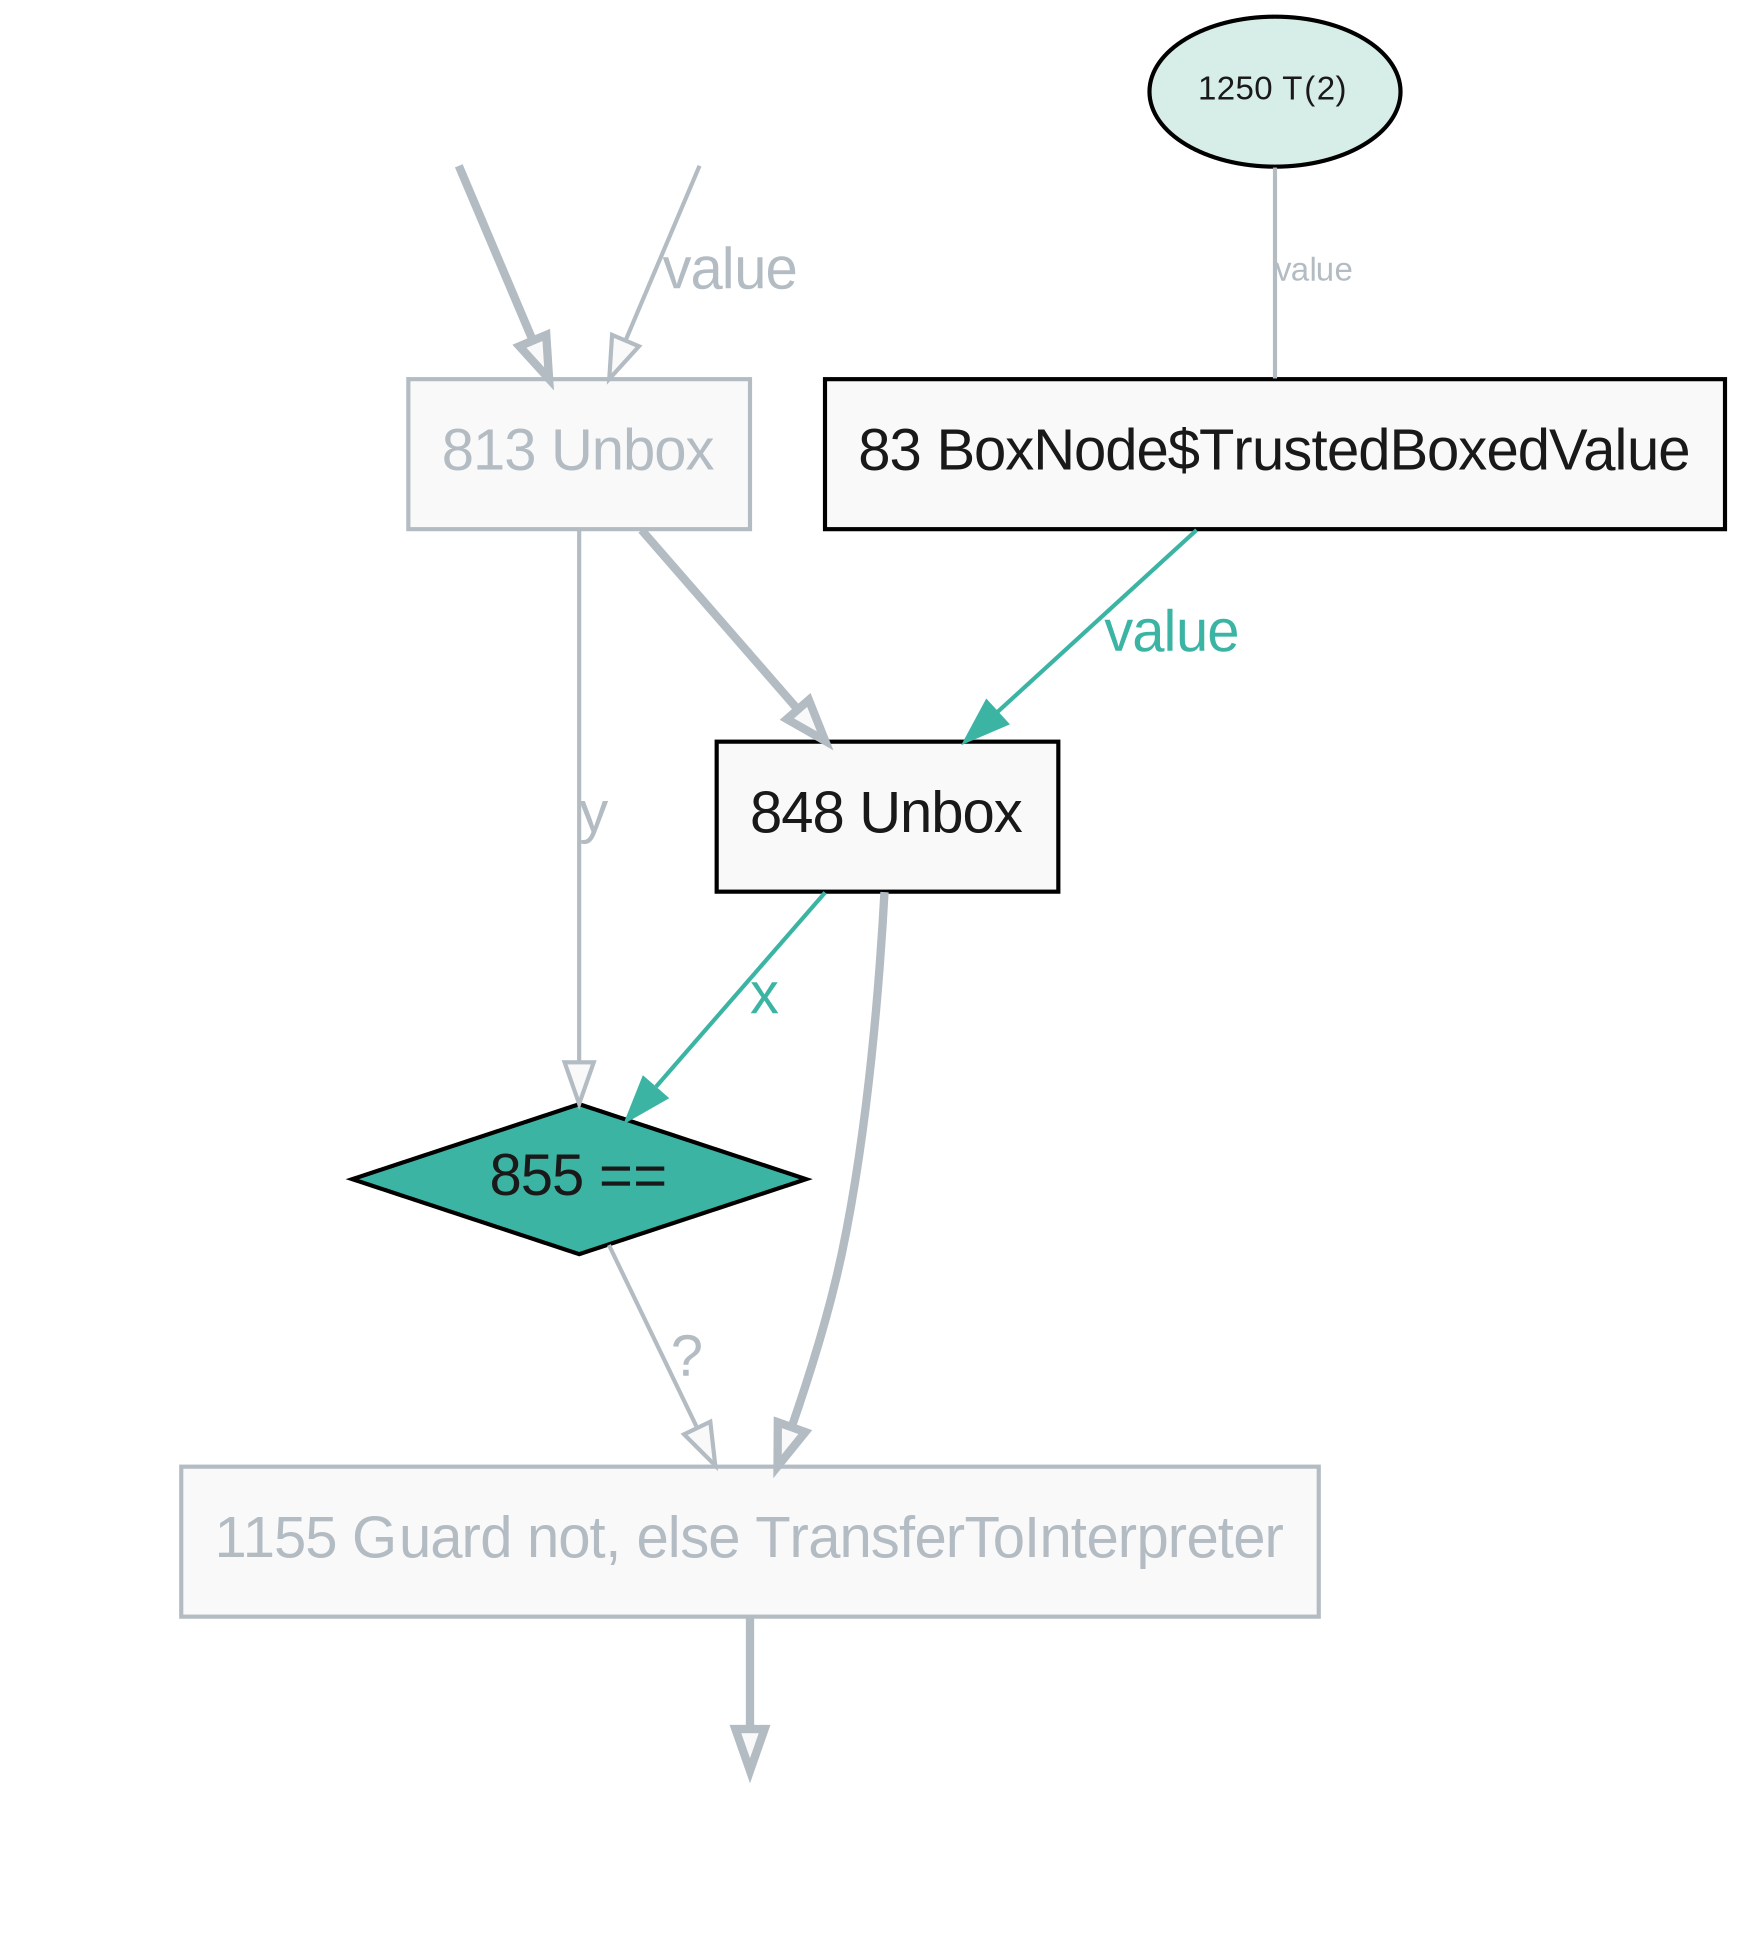
\includegraphics[width=0.4\textwidth]{figures/dot/List.contains.boxed-param-read.TruffleTier.png}
	\caption{Graal IR with speculative unboxing of \scalainline{elem} based on a type profile of its frame slot in \scalainline{List.contains}}
	\label{graalir:cons-contains-param-read}
\end{figure}

As previously mentioned, Truffle can speculatively optimize read operations on boxed frame values.
Figure \ref{graalir:cons-contains-param-read}, contains the parameter of \scalainline{elem} in \scalainline{List.contains}, which is an example of such a speculative optimization.
This speculative optimization relies on a \javainline{TrustedBoxedValue} to unbox the primitive.
A \javainline{TrustedBoxedValue} represents injected information from an external source.

In this particular case, it is known by the compiler that the boxed instance comes from the invocation \scalainline{List.contains((elem: Int))}.
Unique \javainline{int} values may be mapped to a unique \javainline{Integer} instance in the Java runtime, eliminating unnecessary boxed object creation.
The unbox operation in node $848$ will be `floated' up the graph such that all subsequent nodes dominated by the reading of a boxed frame value have no autoboxing.

This optimization is also possible because the invocation of \scalainline{contains} occurs in a single type context.
That is, \scalainline{contains} is only ever invoked with a single type argument in our microbenchmark; therefore, Truffle can insert speculative optimizations based on the type of the argument passed.
As the number of types is limited, in our case, only a single type, the value can be speculatively unboxed.
This optimization would \textit{not} be possible in a multiple type context, where \scalainline{contains} is invoked at many sites with distinct value type arguments.
This type of invocation environment, more commonly found in real-world programs, pollutes the type profiles of the method and inhibits speculative unboxing operations.
In theory, our approach to method specialization would not be hindered by this problem; we consider the evaluation of the interpreter in this environment out of the scope of this thesis.

\begin{figure}[!htb]
	\centering
	\begin{subfigure}[b]{0.4\textwidth}
		\centering
		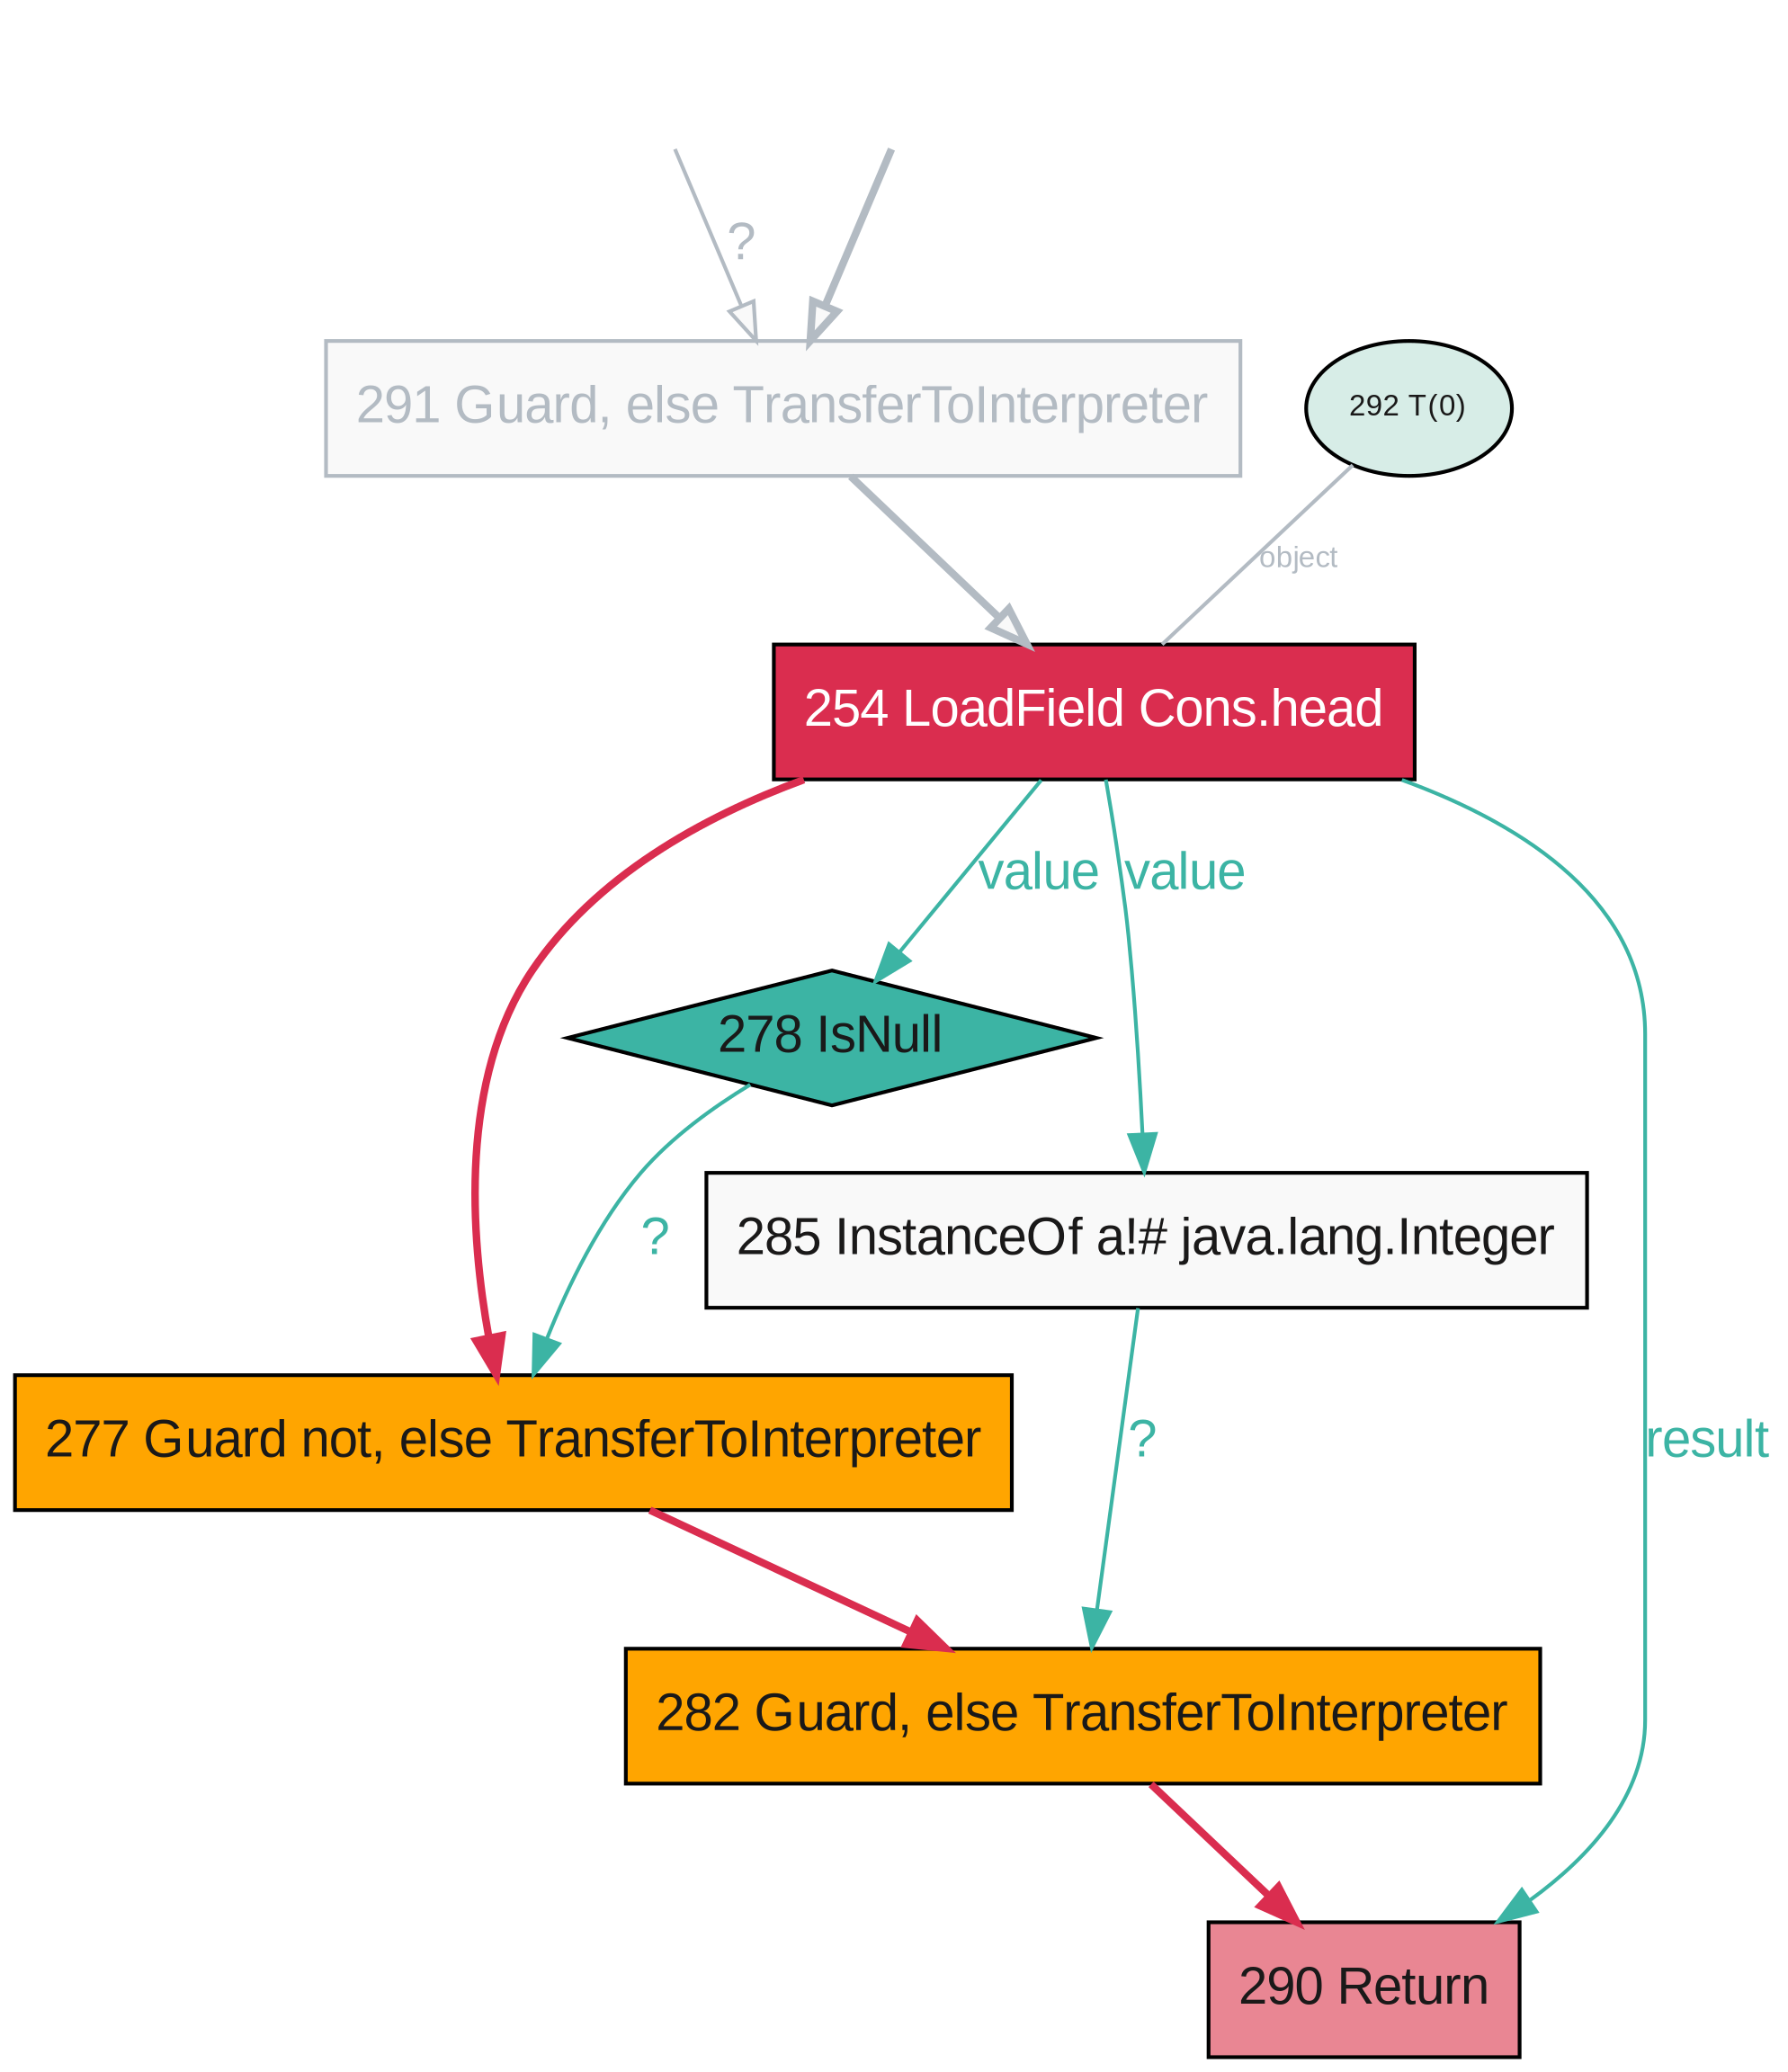
\includegraphics[width=\textwidth]{figures/dot/List.head.boxed.TruffleTier.png}
		\caption{Graal IR of \scalainline{Cons.head} focused on field access of \scalainline{head0}}
		\label{graalir:cons-head-boxed}
	\end{subfigure}
	\hfill
	\begin{subfigure}[b]{0.45\textwidth}
		\centering
		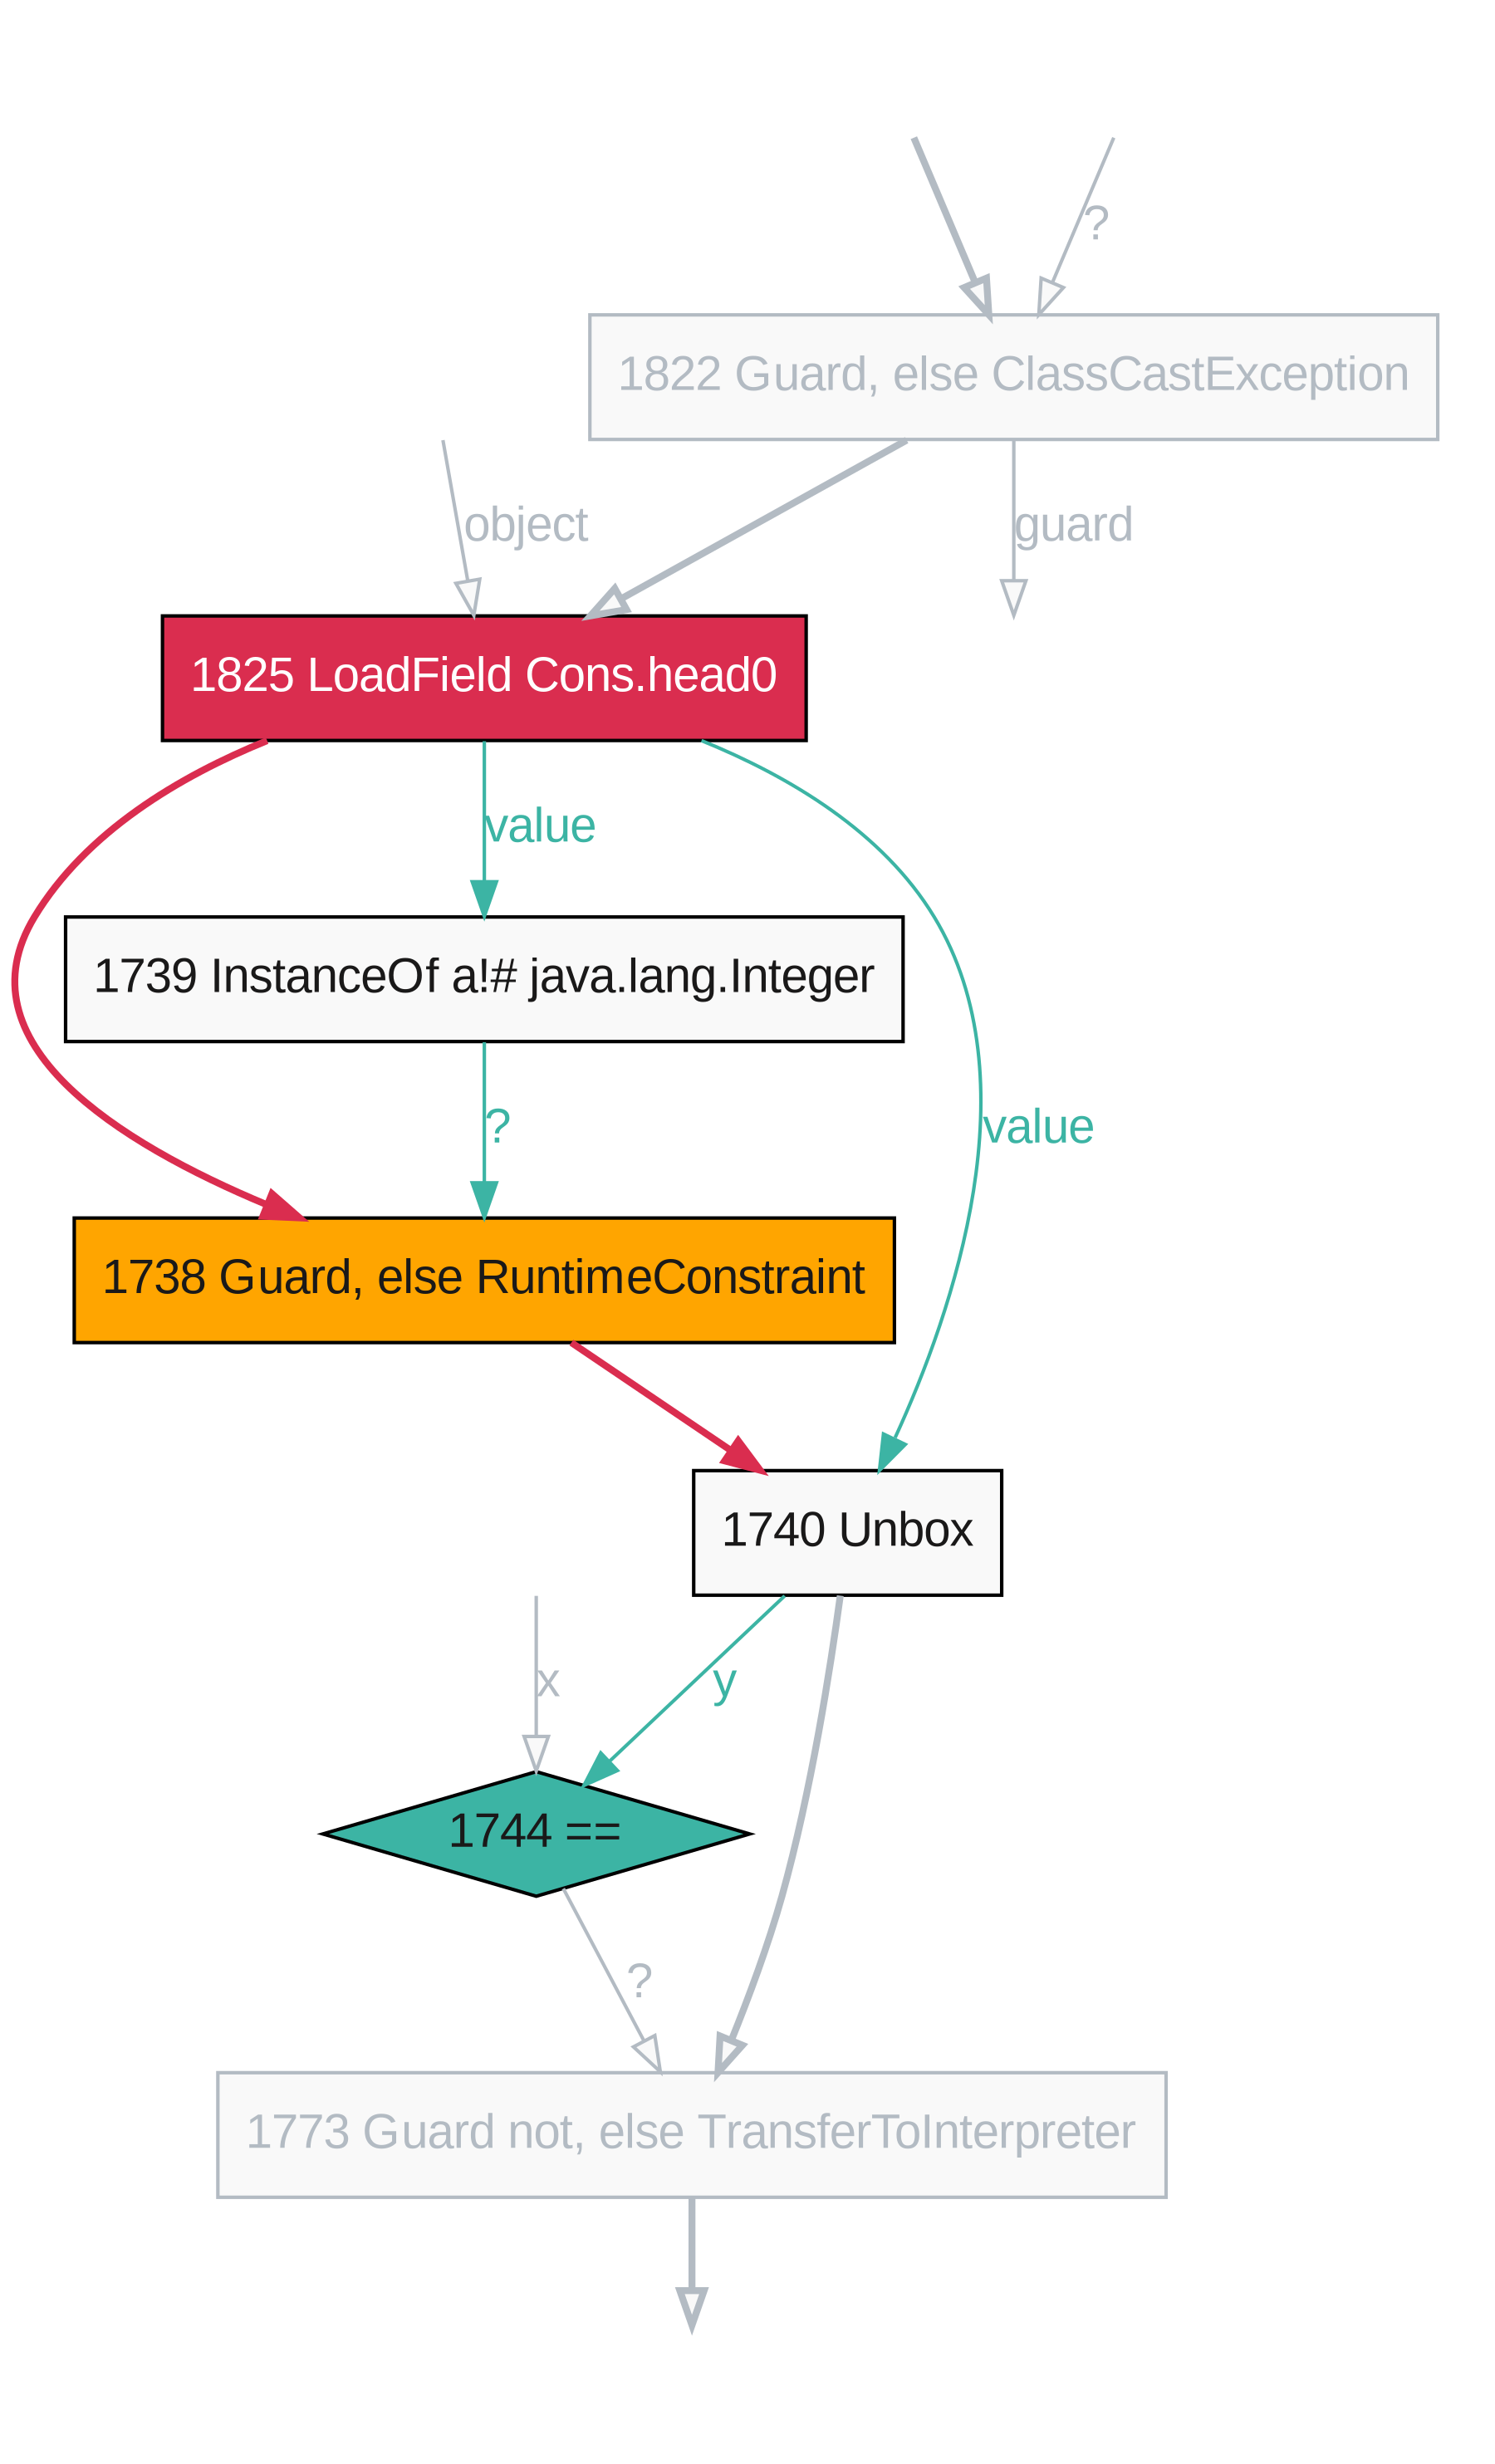
\includegraphics[width=\textwidth]{figures/dot/List.contains.boxed.TruffleTier.png}
		\caption{Graal IR of \scalainline{Cons.head} after being inlined into \scalainline{Cons.contains}}
		\label{graalir:cons-contains-head-focus-boxed}
	\end{subfigure}
	\hfill
\end{figure}

We examine in detail the Graal IR focusing on the \scalainline{List.head} accessor method in our \scalainline{List} running example.
The accessor is frequently used in our \scalainline{List} microbenchmarks; Performance of \scalainline{List.contains} and \scalainline{List.hashCode} depends on the elimination of the unboxing in this method.
We focus on unboxing when the \scalainline{head} field is accessed by the \scalainline{List.head} accessor.
This unboxing can be seen in \ref{graalir:cons-head-boxed}.

We can see that \textit{guard} nodes are inserted by Graal into the compiled graph during JIT compilation.
A guard node ensures that a speculative assumption still holds during execution.
Because the default storage type of a polymorphic field without specialization is an \javainline{Object}, Graal makes two runtime assumptions about the field in the JIT compiled \scalainline{contains} method to ensure the compiled method does not throw a runtime exception if the return value needs to be unboxed.
The first guard, identifiable by node $278$, checks that the value is not the \javainline{null} reference.
As the \javainline{null} value is only compatible with reference types, attempting to unbox a \javainline{null} value produces a runtime exception.
The second guard, with the identifier $282$, is a type check that the value is an \javainline{Integer} object.
Notice that the predecessor node is the type check \javainline{instanceof a!{\#} java.lang.Integer} and not \javainline{instanceof java.lang.Integer}.
\javainline{instanceof} nodes in Graal IR checks against \textit{stamps} instead of normal JVM types identifiers.
A stamp is much like a type identifier but has additional descriptors attached.
For example, the stamp \javainline{a!{\#} java.lang.Integer} has the following descriptors:

\begin{description}
	\item[\texttt{(a)}] Asserts that the stamp marks a reference type identifier. In the case of this stamp, the stamp marks the boxed reference type \javainline{java.lang.Integer}.
	\item[\texttt{(!)}] Asserts that value is not the \javainline{null} reference value. The stamp contains this descriptor because it is preceded by a non-null guard.
	\item[\texttt{(\#)}] Asserts that value marked by the stamp is \textit{exactly} an instance of the type identifier described by the stamp and not an instance of a subclass of the type identifier
\end{description}

In more succinct terms, the \javainline{instanceof} node $285$ checks that value is precisely the instance of a \javainline{java.lang.Integer} and is not the \javainline{null} value. 
If the assumptions are not violated in compiled code, the boxed integer value is then returned from the compiled code.
Note that no unboxing happens because the value of \scalainline{head} has not yet been used in a polymorphic context.

\begin{figure}[!htb]
	\centering
	\begin{subfigure}[b]{0.4\textwidth}
		\centering
		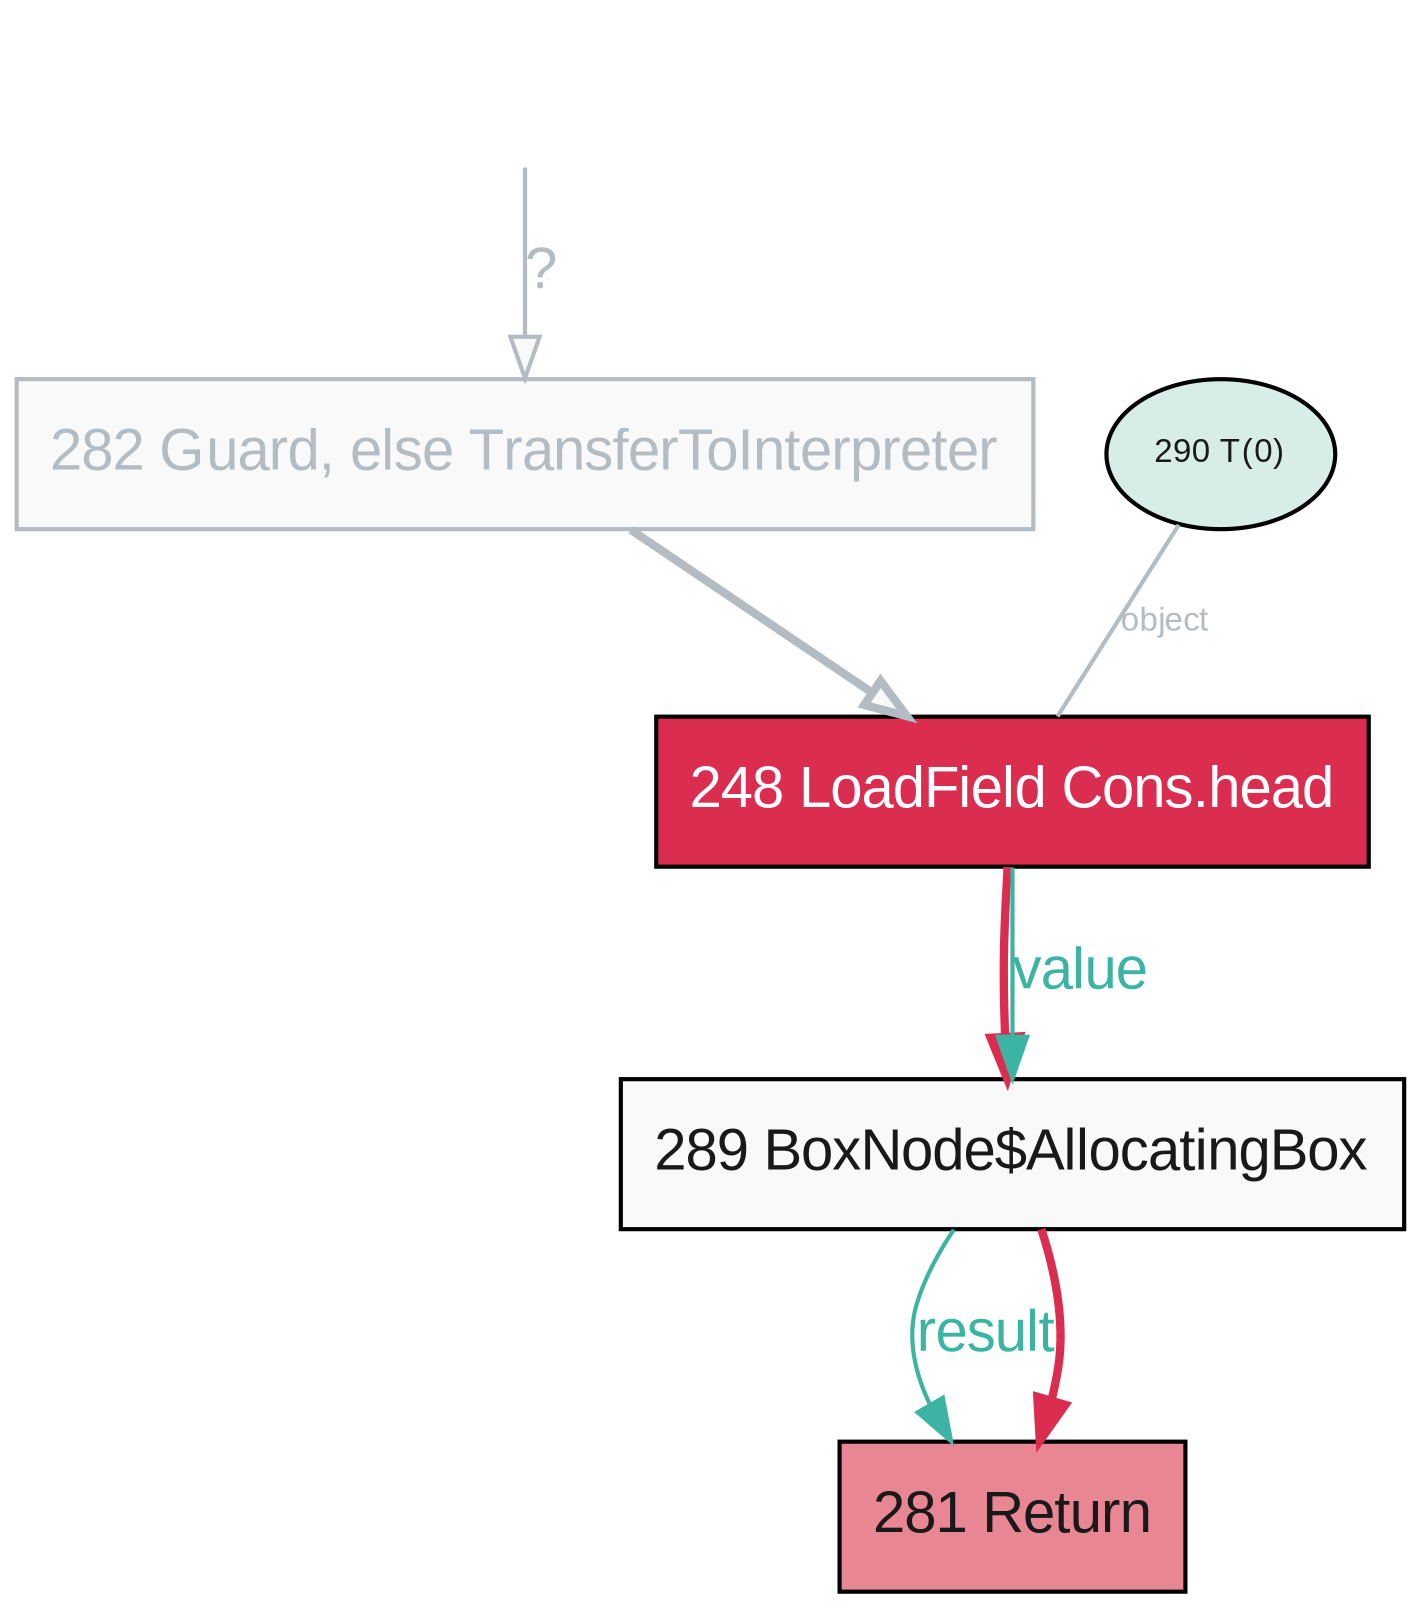
\includegraphics[width=\textwidth]{figures/dot/List.head.specialized.TruffleTier.png}
		\caption{Graal IR of \scalainline{List.head} after field read of \scalainline{head} is specialized.}
		\label{graalir:cons-head-specialized}
	\end{subfigure}
	\hfill
	\begin{subfigure}[b]{0.4\textwidth}
		\centering
		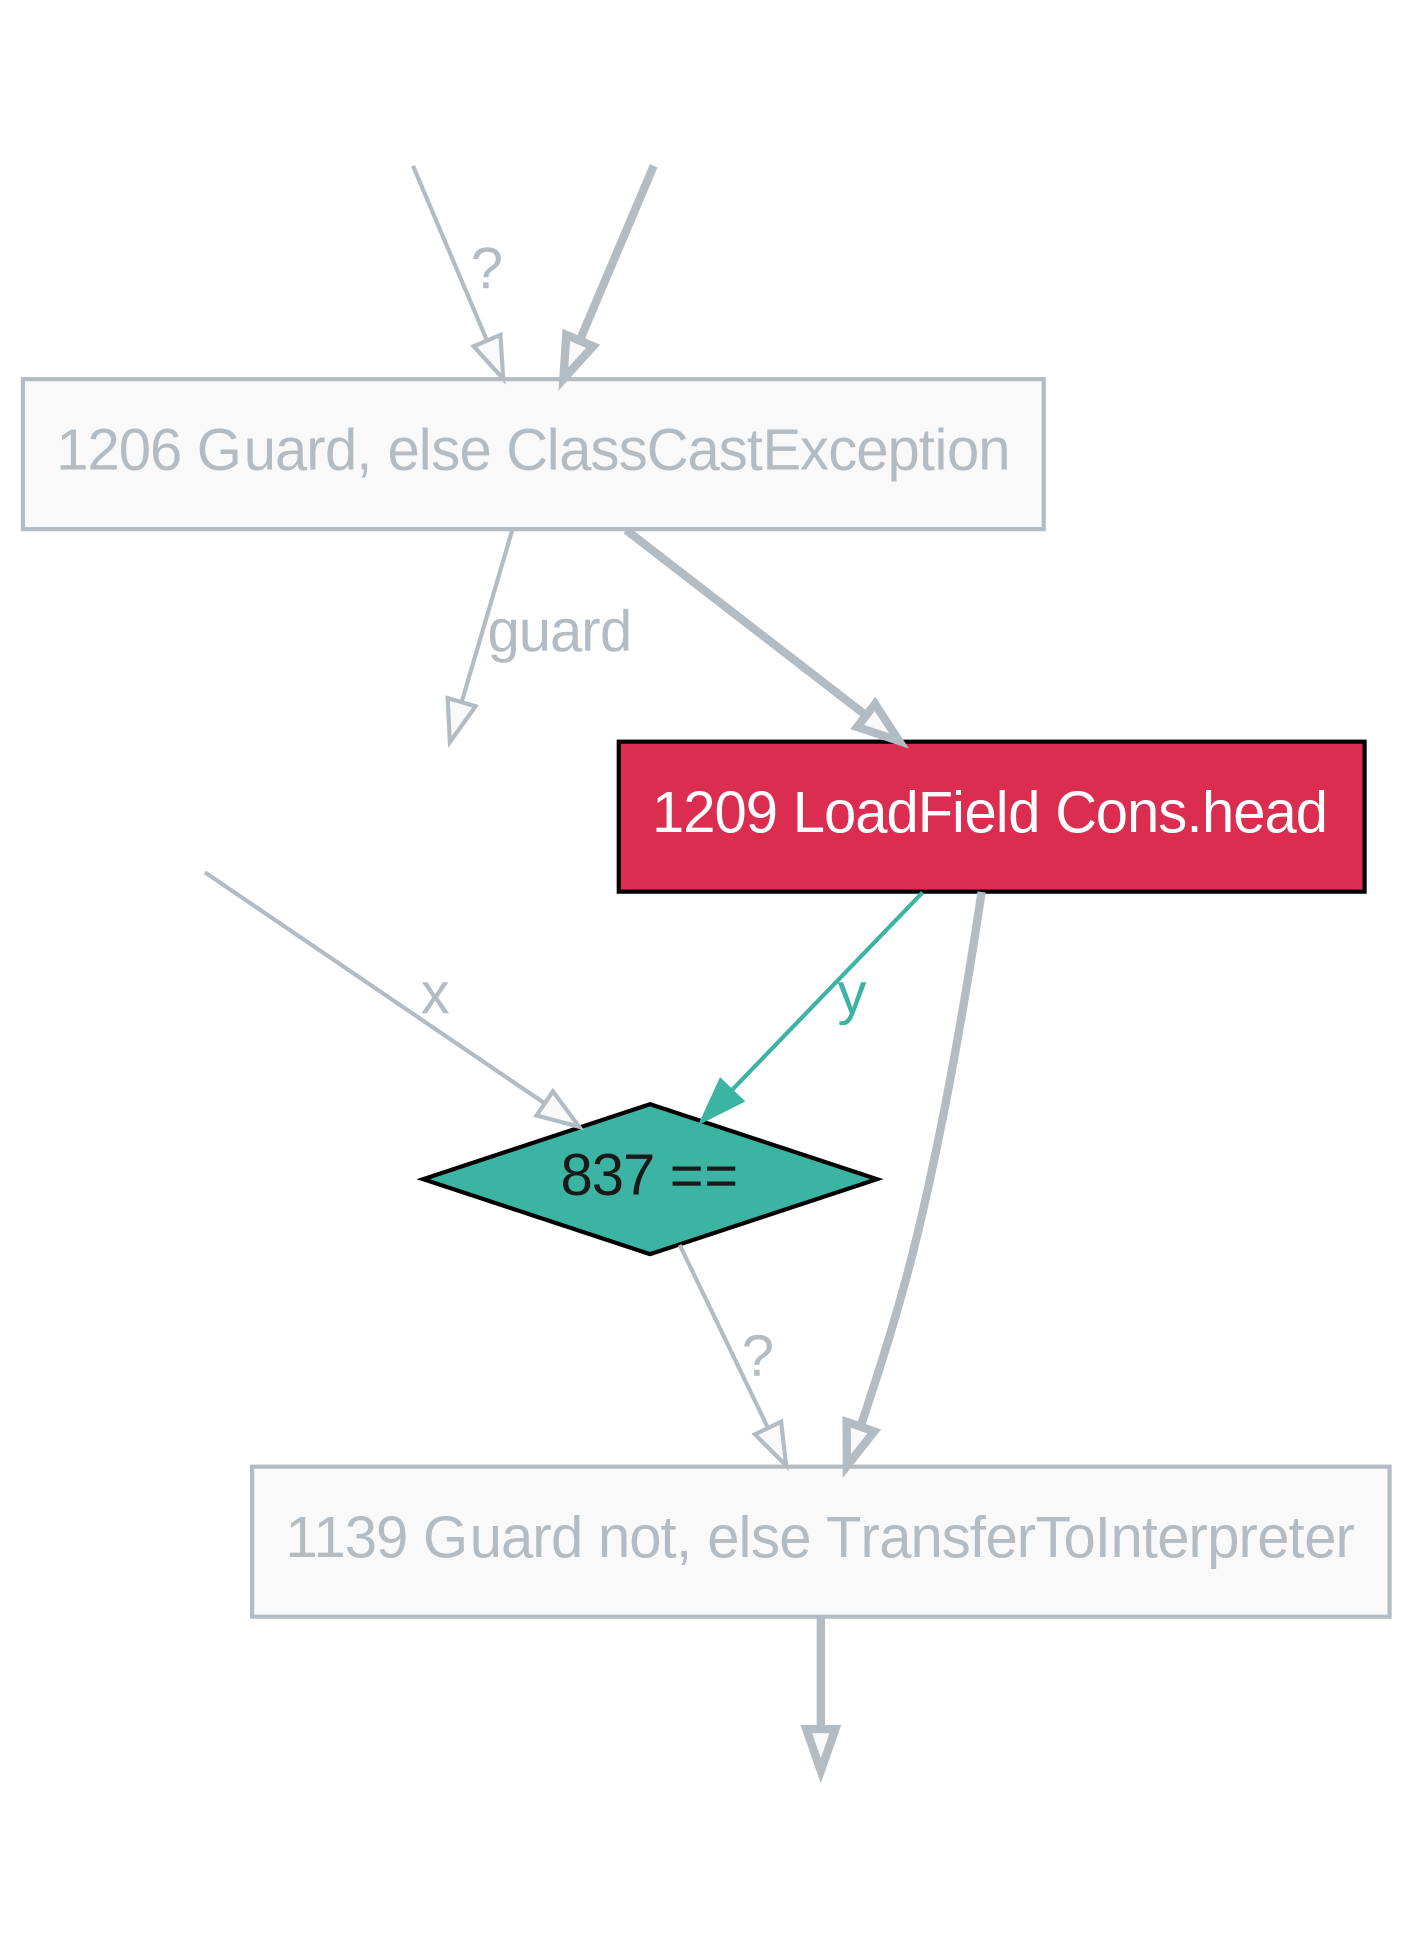
\includegraphics[width=\textwidth]{figures/dot/List.contains.specialized.TruffleTier.png}
		\caption{Graal IR of \scalainline{Cons.head} after being inlined into \scalainline{Cons.contains}}
		\label{graalir:cons-contains-head-focus-specialized}
	\end{subfigure}
	\hfill
\end{figure}

When the access or method \scalainline{List.head} is inlined into its callsite in \scalainline{Cons.contains} (see figure \ref{graalir:cons-contains-head-focus-boxed}), an unbox operation is introduced because the equality operation in node $1744$ compares primitives and not references.
Notice that the two guards nodes previously seen in figure \ref{graalir:cons-head-boxed} are folded into one node because the \javainline{instanceof} node is an extension of the null check node.
Because polymorphic field values are stored as a reference on the object instance, these speculative assumptions are necessary to generate compiled code.
To eliminate the overhead of the unbox operation and the accompanying guard nodes, The polymorphic fields of a class must be specialized.

Figure \ref{graalir:cons-head-specialized} contains the field access of \scalainline{head} after the field has been specialized and has the appropriate storage type in the storage layout of \scalainline{Cons[Int]}.
Notice that a box node has been introduced prior to the value of \scalainline{head} prior to the return node of \scalainline{Cons.head}.
Because the \scalainline{execute} method of a \scalainline{DefDefNode} returns an \javainline{Object}, the return value is preemptively boxed when inspecting the IR of the method.
However, after inlining into the body of \scalainline{Cons.contains}, the box operation is no longer necessary as the boxed value will be immediately unboxed.
Graal will automatically eliminate this type of autoboxing.
When a specialized class instance is used in place of a generic class instance, the field access subgraph of \scalainline{List.head} is fully simplified.

\subsection{Mixing in Array Type Information}

While eliminating the autoboxing of frame and field accesses provided incremental improvements, incorporating array type information atop produced further throughput improvements for our array-backed microbenchmark.
In this subsection, we examine the Graal IR that contain type switches for the Scala runtime to handle arrays.

\begin{figure}[!htb]
	\centering
	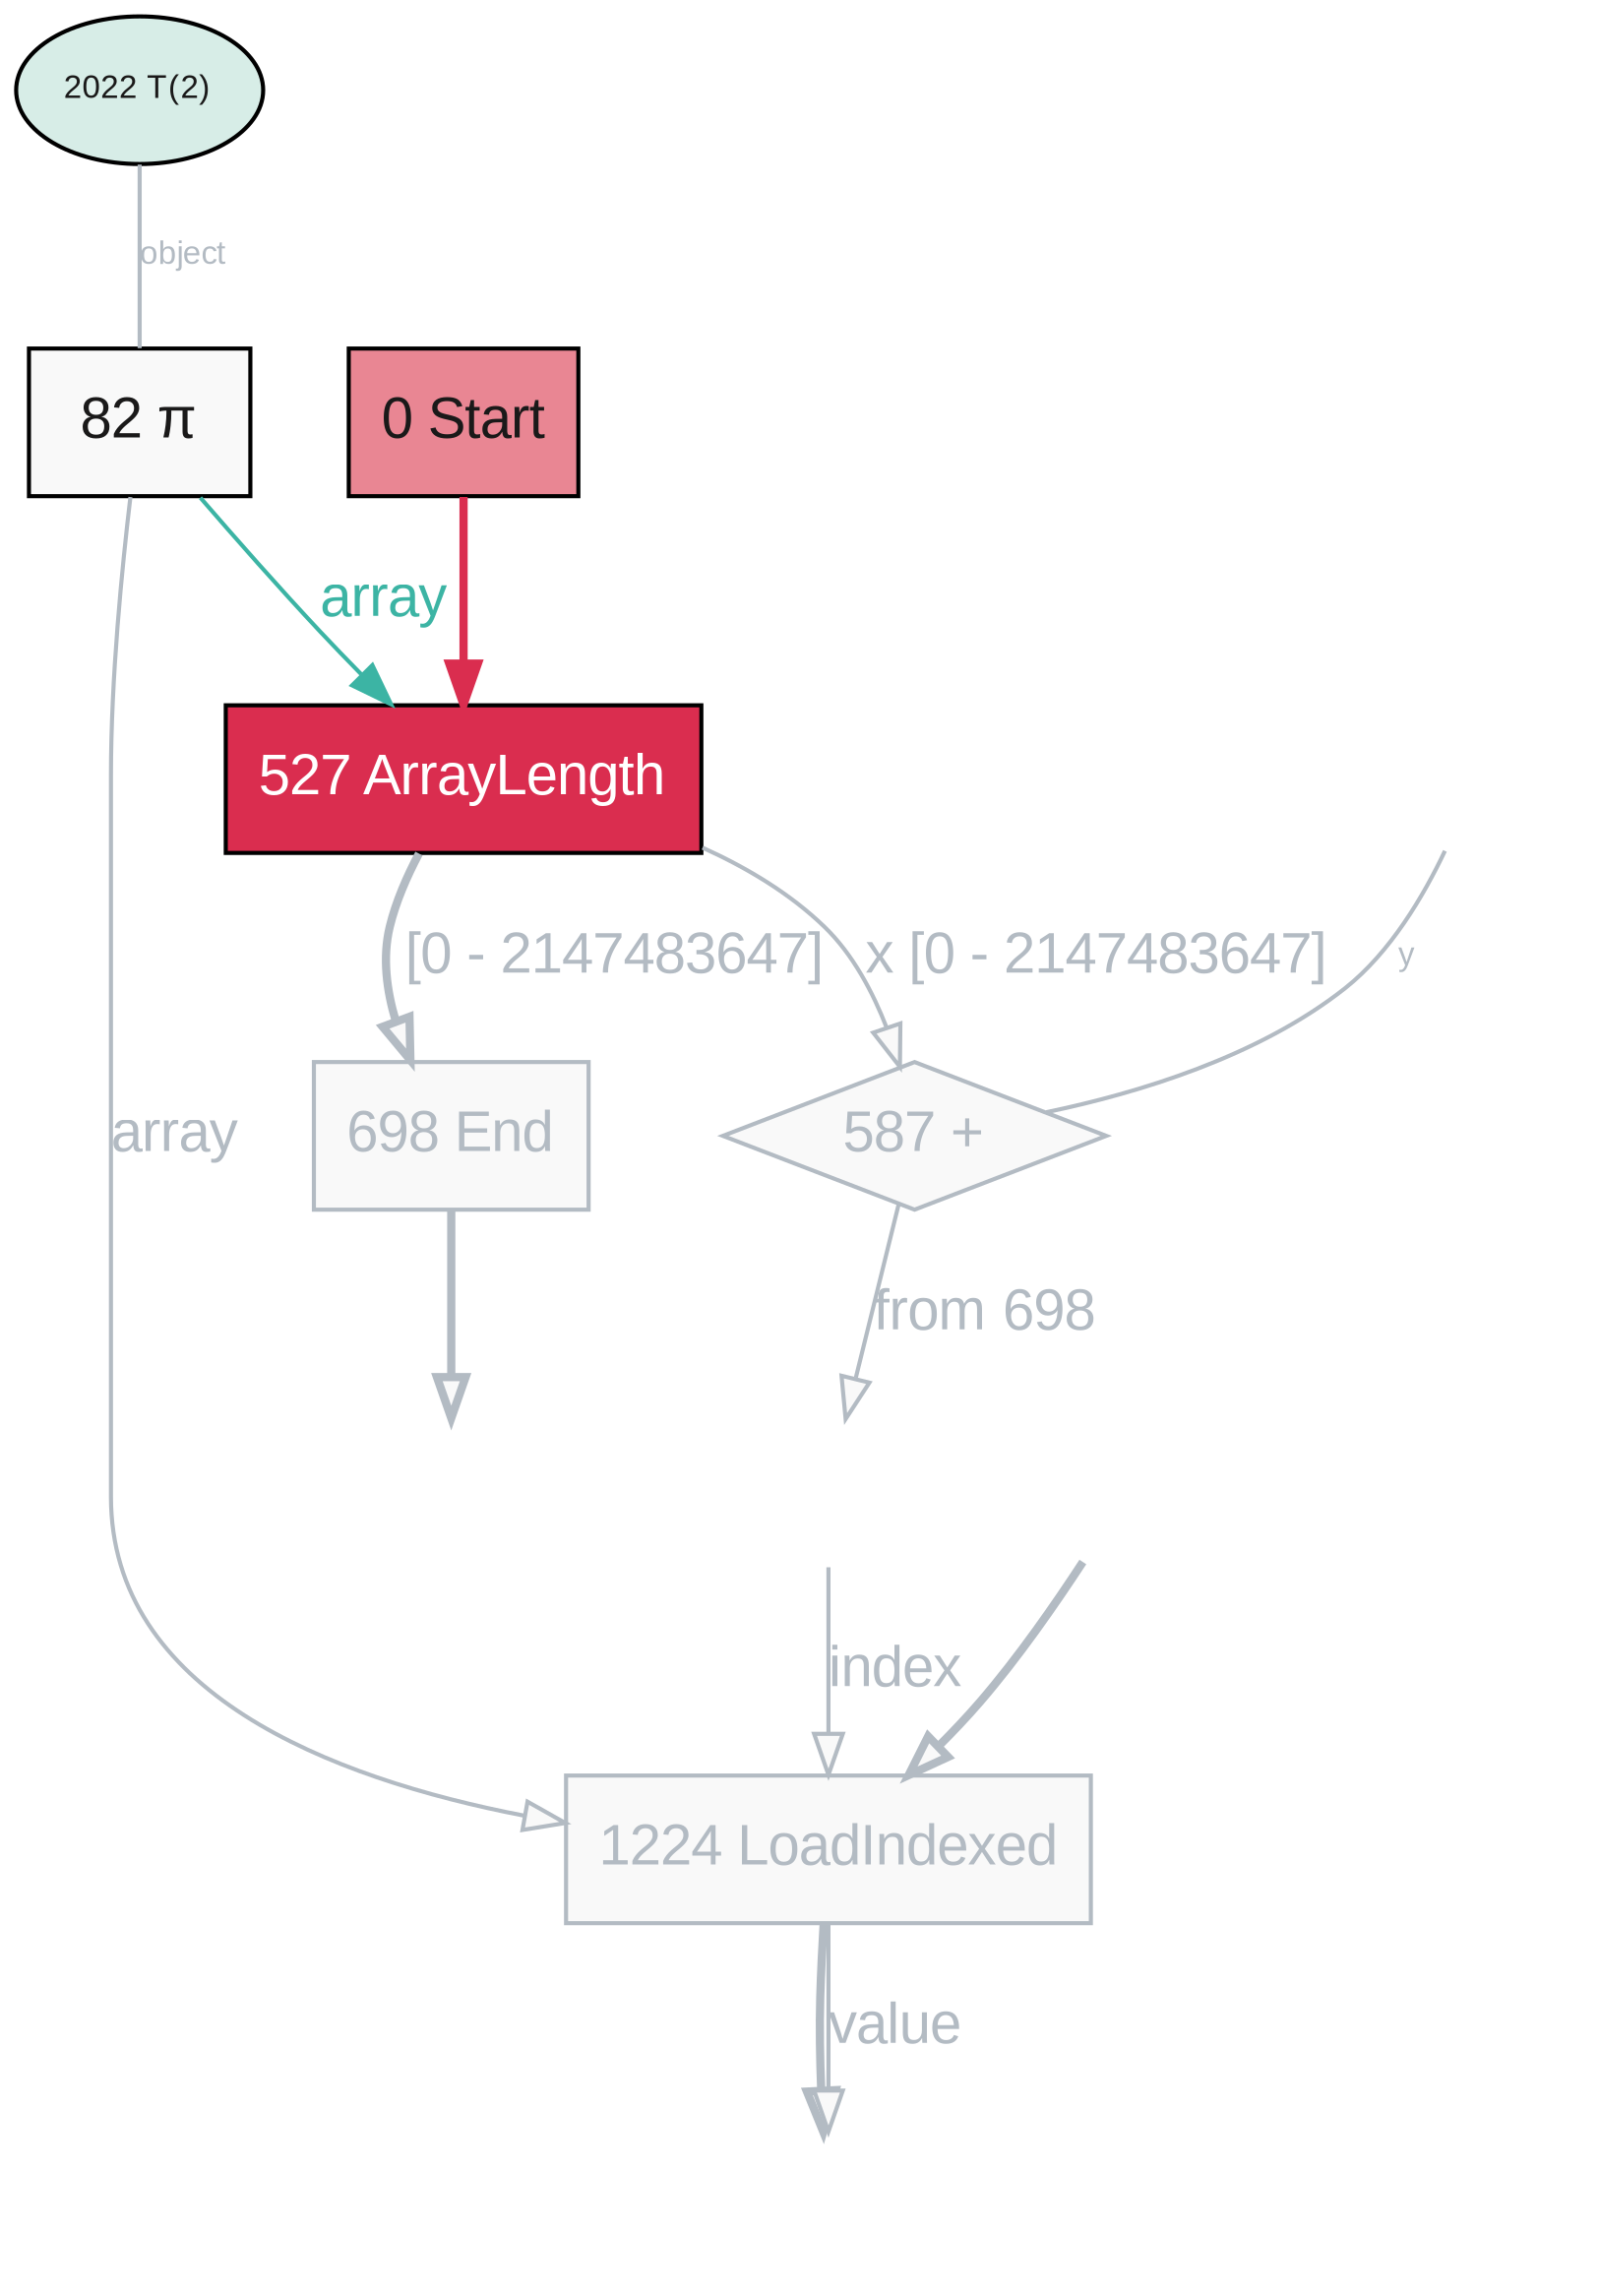
\includegraphics[width=0.3\textwidth]{figures/dot/List.apply.specialized.array_length.png}
	\caption{Graal IR of \scalainline{array_length} in the context of \scalainline{List.apply[T](array: Array[T])} augmented with a $\pi$ node}
	\label{graalir:list-apply-specialized-array-length}
\end{figure}

Figure \ref{graalir:list-apply-boxed-array-length} contains the Graal IR of \scalainline{array_length} inlined into \scalainline{List.apply[T]}. 
Notice that the \scalainline{instanceof} type checks nodes (white) that are succeeded by an \javainline{ArrayLength} node (red) for each of the branches in \scalainline{array_length}.
The numerous consecutive conditional expressions complicate the control flow analysis in JIT compilation.
These conditional checks add unnecessary branching and burdens JIT compilation when the type of a specialized array could be known from specialization.

\begin{figure}
	\centering
	\includegraphics[width=\textwidth]{figures/dot/List.apply.boxed.array_length.png}
	\caption{Graal IR of \scalainline{array_length} in the context of \scalainline{List.apply[T](array: Array[T])}}
	\label{graalir:list-apply-boxed-array-length}
\end{figure}

Figure \ref{graalir:list-apply-specialized-array-length} contains the simplified Graal IR of \scalainline{array_length} inlined into \scalainline{List.apply[T]}.
Notice that there is a single \javainline{ArrayLength} node that is dominated by a $\pi$ node.
A $\pi$ node\cite{abdc:pi-nodes} enforces a bound on a value.
In the case of Graal, a $\pi$ node enforces bound on the type of a value.
More specifically in our example, the $\pi$ node narrows the type of the 2nd parameter of \scalainline{List.apply[T]} to a monomorphic array type.
When the type of the parameter is narrowed, the type checks that enforce array types from figure \ref{graalir:list-apply-boxed-array-length} are eliminated because the type is now known.

This method does not consider polymorphic scenarios where an array of boxed primitives are used interchangeably with an array of primitives.
Such scenarios would require the insertion of additional autoboxing nodes or an intraprocedural transformation where boxed arrays are converted to primitive arrays.
While these solutions are possible in the context of Truffle, we consider these kinds of scenarios out of the scope of this thesis.



